
%(BEGIN_QUESTION)
% Copyright 2006, Tony R. Kuphaldt, released under the Creative Commons Attribution License (v 1.0)
% This means you may do almost anything with this work of mine, so long as you give me proper credit

One of the most fundamental relationships in the study of electricity is {\it Ohm's Law}.  This mathematical expression relates the flow of electric charge ($I$, which we call {\it current}) to electromotive potential ($V$, which we call {\it voltage}) and opposition to charge flow ($R$, which we call {\it resistance}):

$$\includegraphics[width=15.5cm]{i00087x01.eps} I = {V \over R} \hbox{\hskip 10pt} \hbox{(For all conditions)}$$

The relationship between {\bf gas} flow rate, pressure drop, and ``resistance'' for a piping restriction (orifice, throttling valve, pipe bend, etc.) is not as simple.  No single mathematical expression is sufficient to predict flow rates for all conditions:

$$\includegraphics[width=15.5cm]{i00087x02.eps}$$

$$Q = {{P_1 - P_2} \over R_1} = {\Delta P \over R_1} \hbox{\hskip 10pt}  \hbox{Subsonic velocity with small }\Delta P$$

\vskip 10pt

$$Q = \sqrt{{P_1 - P_2} \over R_2} = \sqrt{\Delta P \over R_2} \hbox{\hskip 10pt}  \hbox{Subsonic velocity with moderate }\Delta P$$

\vskip 10pt

$$Q = \sqrt{P_2({P_1 - P_2}) \over R_3} = \hbox{\hskip 10pt}  \hbox{Subsonic velocity with large }\Delta P$$

Shunt resistors may be used as electric current-measuring elements, producing a voltage drop in precise proportion to the current through it.  All we need to know is the shunt resistance, and we may infer current by measuring voltage.  In a similar manner, orifices may be used as gas flow-measuring elements, producing a pressure drop that varies with the amount of flow passing through it:

$$\includegraphics[width=15.5cm]{i00087x03.eps}$$

Given the ``Ohm's Law'' equations shown for gas flow, identify what we would have to know before using an orifice as an accurate gas flow-measuring device, and how we would be able to obtain that information.  Also identify the type of sensing instrument(s) we would need to measure the pressure, so we could infer flow rate from its reading.

\underbar{file i00087}
%(END_QUESTION)





%(BEGIN_ANSWER)

Here, what we do not know about the flow-measurement scenario is the flow regime (laminar or turbulent), and also what the ``resistance'' of the fluid restriction is.  Of course, the Reynolds number for our flowstream will indicate its regime status, and the $R$ factor for the orifice may be either determined experimentally or derived from orifice equations (available in any exhaustive reference book).

\vskip 10pt

The proper pressure-sensing instrument to use for fluid flow is a {\it differential pressure} instrument, such as a DP cell or DP gauge, or perhaps even a mercury manometer.  In the case of large pressure drops, it may also be important to measure downstream pressure ($P_2$) with reference to atmosphere.

%(END_ANSWER)





%(BEGIN_NOTES)

In case anyone asks, I use subscripts to distinguish the ``resistance'' values $R_1$, $R_2$, etc. in order to show that the ``resistance'' factor will be different for each flow regime.

\vskip 10pt

The last equation was derived from a more complex variation found in {\it Control Systems Engineering}, by William J. Palm (published by John Wiley \& Sons, copyright 1986):

$$q = C_d A \sqrt{{ 2 \over {R_g T_1}} P_2(P_1 - P_2)}$$

This same author states that the gas flow will be subsonic if the absolute pressure ratio ${P_1 \over P_2} < 1.894$.  A good rule-of-thumb I have read in B\'ela Lipt\'ak's {\it Instrument Engineer's Handbook, Process Control} is that the gas flow {\it will} be supersonic if the absolute upstream pressure is twice that (or more) of the absolute downstream pressure.

%INDEX% Physics, dynamic fluids: Resistance of gas flow component

%(END_NOTES)


